%% http://www.ieee.org/


\documentclass[conference]{IEEEtran}

% *** CITATION PACKAGES ***
%
\usepackage{cite}
% cite.sty was written by Donald Arseneau
% V1.6 and later of IEEEtran pre-defines the format of the cite.sty package
% \cite{} output to follow that of the IEEE. Loading the cite package will
% result in citation numbers being automatically sorted and properly
% "compressed/ranged". e.g., [1], [9], [2], [7], [5], [6] without using
% cite.sty will become [1], [2], [5]--[7], [9] using cite.sty. cite.sty's
% \cite will automatically add leading space, if needed. Use cite.sty's
% noadjust option (cite.sty V3.8 and later) if you want to turn this off
% such as if a citation ever needs to be enclosed in parenthesis.
% cite.sty is already installed on most LaTeX systems. Be sure and use
% version 5.0 (2009-03-20) and later if using hyperref.sty.
% The latest version can be obtained at:
% http://www.ctan.org/pkg/cite
% The documentation is contained in the cite.sty file itself.



% *** GRAPHICS RELATED PACKAGES ***
%
\ifCLASSINFOpdf
  % \usepackage[pdftex]{graphicx}
  % declare the path(s) where your graphic files are
  % \graphicspath{{../pdf/}{../jpeg/}}
  % and their extensions so you won't have to specify these with
  % every instance of \includegraphics
  % \DeclareGraphicsExtensions{.pdf,.jpeg,.png}
\else
  % or other class option (dvipsone, dvipdf, if not using dvips). graphicx
  % will default to the driver specified in the system graphics.cfg if no
  % driver is specified.
  % \usepackage[dvips]{graphicx}
  % declare the path(s) where your graphic files are
  % \graphicspath{{../eps/}}
  % and their extensions so you won't have to specify these with
  % every instance of \includegraphics
  % \DeclareGraphicsExtensions{.eps}
\fi
% graphicx was written by David Carlisle and Sebastian Rahtz. It is
% required if you want graphics, photos, etc. graphicx.sty is already
% installed on most LaTeX systems. The latest version and documentation
% can be obtained at: 
% http://www.ctan.org/pkg/graphicx
% Another good source of documentation is "Using Imported Graphics in
% LaTeX2e" by Keith Reckdahl which can be found at:
% http://www.ctan.org/pkg/epslatex
%
% latex, and pdflatex in dvi mode, support graphics in encapsulated
% postscript (.eps) format. pdflatex in pdf mode supports graphics
% in .pdf, .jpeg, .png and .mps (metapost) formats. Users should ensure
% that all non-photo figures use a vector format (.eps, .pdf, .mps) and
% not a bitmapped formats (.jpeg, .png). The IEEE frowns on bitmapped formats
% which can result in "jaggedy"/blurry rendering of lines and letters as
% well as large increases in file sizes.
%
% You can find documentation about the pdfTeX application at:
% http://www.tug.org/applications/pdftex





% *** MATH PACKAGES ***
%
\usepackage{amsmath}
% A popular package from the American Mathematical Society that provides
% many useful and powerful commands for dealing with mathematics.
%
% Note that the amsmath package sets \interdisplaylinepenalty to 10000
% thus preventing page breaks from occurring within multiline equations. Use:
%\interdisplaylinepenalty=2500
% after loading amsmath to restore such page breaks as IEEEtran.cls normally
% does. amsmath.sty is already installed on most LaTeX systems. The latest
% version and documentation can be obtained at:
% http://www.ctan.org/pkg/amsmath





% *** SPECIALIZED LIST PACKAGES ***
%
%\usepackage{algorithmic}
% algorithmic.sty was written by Peter Williams and Rogerio Brito.
% This package provides an algorithmic environment fo describing algorithms.
% You can use the algorithmic environment in-text or within a figure
% environment to provide for a floating algorithm. Do NOT use the algorithm
% floating environment provided by algorithm.sty (by the same authors) or
% algorithm2e.sty (by Christophe Fiorio) as the IEEE does not use dedicated
% algorithm float types and packages that provide these will not provide
% correct IEEE style captions. The latest version and documentation of
% algorithmic.sty can be obtained at:
% http://www.ctan.org/pkg/algorithms
% Also of interest may be the (relatively newer and more customizable)
% algorithmicx.sty package by Szasz Janos:
% http://www.ctan.org/pkg/algorithmicx




% *** ALIGNMENT PACKAGES ***
%
%\usepackage{array}
% Frank Mittelbach's and David Carlisle's array.sty patches and improves
% the standard LaTeX2e array and tabular environments to provide better
% appearance and additional user controls. As the default LaTeX2e table
% generation code is lacking to the point of almost being broken with
% respect to the quality of the end results, all users are strongly
% advised to use an enhanced (at the very least that provided by array.sty)
% set of table tools. array.sty is already installed on most systems. The
% latest version and documentation can be obtained at:
% http://www.ctan.org/pkg/array


% IEEEtran contains the IEEEeqnarray family of commands that can be used to
% generate multiline equations as well as matrices, tables, etc., of high
% quality.




% *** SUBFIGURE PACKAGES ***
%\ifCLASSOPTIONcompsoc
%  \usepackage[caption=false,font=normalsize,labelfont=sf,textfont=sf]{subfig}
%\else
%  \usepackage[caption=false,font=footnotesize]{subfig}
%\fi
% subfig.sty, written by Steven Douglas Cochran, is the modern replacement
% for subfigure.sty, the latter of which is no longer maintained and is
% incompatible with some LaTeX packages including fixltx2e. However,
% subfig.sty requires and automatically loads Axel Sommerfeldt's caption.sty
% which will override IEEEtran.cls' handling of captions and this will result
% in non-IEEE style figure/table captions. To prevent this problem, be sure
% and invoke subfig.sty's "caption=false" package option (available since
% subfig.sty version 1.3, 2005/06/28) as this is will preserve IEEEtran.cls
% handling of captions.
% Note that the Computer Society format requires a larger sans serif font
% than the serif footnote size font used in traditional IEEE formatting
% and thus the need to invoke different subfig.sty package options depending
% on whether compsoc mode has been enabled.
%
% The latest version and documentation of subfig.sty can be obtained at:
% http://www.ctan.org/pkg/subfig




% *** FLOAT PACKAGES ***
%
%\usepackage{fixltx2e}
% fixltx2e, the successor to the earlier fix2col.sty, was written by
% Frank Mittelbach and David Carlisle. This package corrects a few problems
% in the LaTeX2e kernel, the most notable of which is that in current
% LaTeX2e releases, the ordering of single and double column floats is not
% guaranteed to be preserved. Thus, an unpatched LaTeX2e can allow a
% single column figure to be placed prior to an earlier double column
% figure.
% Be aware that LaTeX2e kernels dated 2015 and later have fixltx2e.sty's
% corrections already built into the system in which case a warning will
% be issued if an attempt is made to load fixltx2e.sty as it is no longer
% needed.
% The latest version and documentation can be found at:
% http://www.ctan.org/pkg/fixltx2e


%\usepackage{stfloats}
% stfloats.sty was written by Sigitas Tolusis. This package gives LaTeX2e
% the ability to do double column floats at the bottom of the page as well
% as the top. (e.g., "\begin{figure*}[!b]" is not normally possible in
% LaTeX2e). It also provides a command:
%\fnbelowfloat
% to enable the placement of footnotes below bottom floats (the standard
% LaTeX2e kernel puts them above bottom floats). This is an invasive package
% which rewrites many portions of the LaTeX2e float routines. It may not work
% with other packages that modify the LaTeX2e float routines. The latest
% version and documentation can be obtained at:
% http://www.ctan.org/pkg/stfloats
% Do not use the stfloats baselinefloat ability as the IEEE does not allow
% \baselineskip to stretch. Authors submitting work to the IEEE should note
% that the IEEE rarely uses double column equations and that authors should try
% to avoid such use. Do not be tempted to use the cuted.sty or midfloat.sty
% packages (also by Sigitas Tolusis) as the IEEE does not format its papers in
% such ways.
% Do not attempt to use stfloats with fixltx2e as they are incompatible.
% Instead, use Morten Hogholm'a dblfloatfix which combines the features
% of both fixltx2e and stfloats:
%
% \usepackage{dblfloatfix}
% The latest version can be found at:
% http://www.ctan.org/pkg/dblfloatfix




% *** PDF, URL AND HYPERLINK PACKAGES ***
%
\usepackage{url}
%\usepackage{amsmath} %create equations in the document
% correct bad hyphenation here
\hyphenation{op-tical net-works semi-conduc-tor}



\usepackage{graphicx} % support the \includegraphics command and options
\usepackage{hyperref}
\usepackage{amsmath}
\usepackage{float}
\usepackage{listings} %so you can write computer code in the LaTex document. 
\begin{document} 
\title{Reducing Audio Bandwidth with an FFT-based Low-Pass Filter}

\author{
    \IEEEauthorblockN{Trent Geisler}
    \IEEEauthorblockA{Analytics and Data Science\\
    Kennesaw State University\\
    Kennesaw, Georgia 30144\\
    }
    \and
    \IEEEauthorblockN{Andrew Henshaw}
    \IEEEauthorblockA{Analytics and Data Science\\
    Kennesaw State University\\
    Kennesaw, Georgia 30144\\
    }
    \and
    \IEEEauthorblockN{Lauren Staples}
    \IEEEauthorblockA{Analytics and Data Science\\
    Kennesaw State University\\
    Kennesaw, Georgia 30144\\
    }
}

\maketitle

\begin{abstract}
The abstract goes here.
\end{abstract}

\IEEEpeerreviewmaketitle

\section{Introduction} 

Filtering an audio signal is extremely important for many
reasons. When an appropriate filter is designed and used to
remove any unwanted frequencies, then the bandwidth and power
necessary for audio signal transmission is reduced. Why is this
important? The frequency bands used for the transmission of many
types of signals are scarce resources. Every transmitter that can
interfere with others has to operate in a licensed band and is
subject to bandwidth limitations. This is why multiple radio
stations can operate in the same geographical area. They are
assigned different center frequencies and they have a certain
bandwidth they can occupy. If one radio station transmits beyond
their assigned bandwidth, they will impact the signal
transmission of other local radio stations. One way to ensure
that a radio station stays within their assigned bandwidth is
through the use of filtering.\cite{notes:class}  

Additionally, if you travel to a different city, you will find
radio stations that operate at the same frequency as the radio
stations located locally here in Atlanta. This is possible
because radio transmitters are limited in power. With unlimited
power, for example, one could hear FM 106.7 throughout the United
States and no other radio station would be able to use the
frequency 106.7 MHz. But power is limited, and high-power radio
transmissions cost a lot of money \cite{notes:class}. This is why
some radio stations like to brag about how powerful their
transmissions are. It is also why start-up radio stations have a
very limited range. Therefore, if power costs money, one does not
want to waste it by broadcasting frequencies that most humans
cannot hear.

Both bandwidth and power savings are the motivation behind Fast
Fourier Transform (FFT)-based low-pass filters. This paper will
demonstrate how a Finite Impulse Response (FIR) low pass filter
can remove unnecessary frequencies in order to reduce the
bandwidth and power required for transmission.  

\subsection{Objective}

Our objective is to design and demonstrate an FFT-based FIR
low-pass filter to reduce bandwidth of a recorded audio signal
for the purposes of AM Radio transmission.

\section{Methods}

We collected data, designed a low pass filter, pushed the signal
through the filter, and then evaluated the resulting signal.

\subsection{Data}
We collected an audio signal by recording the song `Flight of the Bumblebee' at the full frequency spectrum that a compact disc (CD) is recorded at, which is 44.1 kHz. The human ear does not even hear this full spectrum.  This means that there are potential bandwidth `savings' for transmission! This collected audio recording is referred to as the `raw signal.'

\subsection{Filter Design}

The typical Human can only hear frequencies in the range of 20Hz through 20kHz, and this range only decreases as humans age  \cite{human:rg}.  Using the website \url{http://onlinetonegenerator.com/hearingtest.html}, we will test the hearing range of each member listening to our final presentation.  This demonstration will provide a tangible example why appropriate filtering of an audio signal will have little to no impact on the quality of sound that a person hears after the filtering.  

When our project group performed the hearing test, the highest audible frequency was 15kHz.  Since our project group was not able to hear the frequencies above the 15kHz threshold, any low-pass filter that removed the high frequencies above 15kHz would have no impact on the quality of the audio signal that  we would hear.  Recall, removing the unecessary frequencies from an audio signal transmission provides a few nice benefits such as the following: 

\begin{enumerate}
\item It reduces the necessary power for transmission of the audio signal
\item It reduces the necessary bandwidth for transmission
\end{enumerate}

Filtering is the processing of a time-domain signal resulting in some change in that signals original spectral content.  The change is usually the reduction or filtering of unwanted input spectral components.\cite{lyons:intro}.  Given the human threshold for hearing, an obvious opportunity is to apply low-pass filtering in order to transmit audio signals that humans can actually hear with smaller bandwidths.  The ideal low pass filter would completely eliminate all frequencies above a certain cutoff point (in our hearing test example, the cutoff would be at 15kHz) while passing all frequencies below the cutoff point \cite{lowpass:wiki}.       

\begin{figure}[h!]
	\centering
	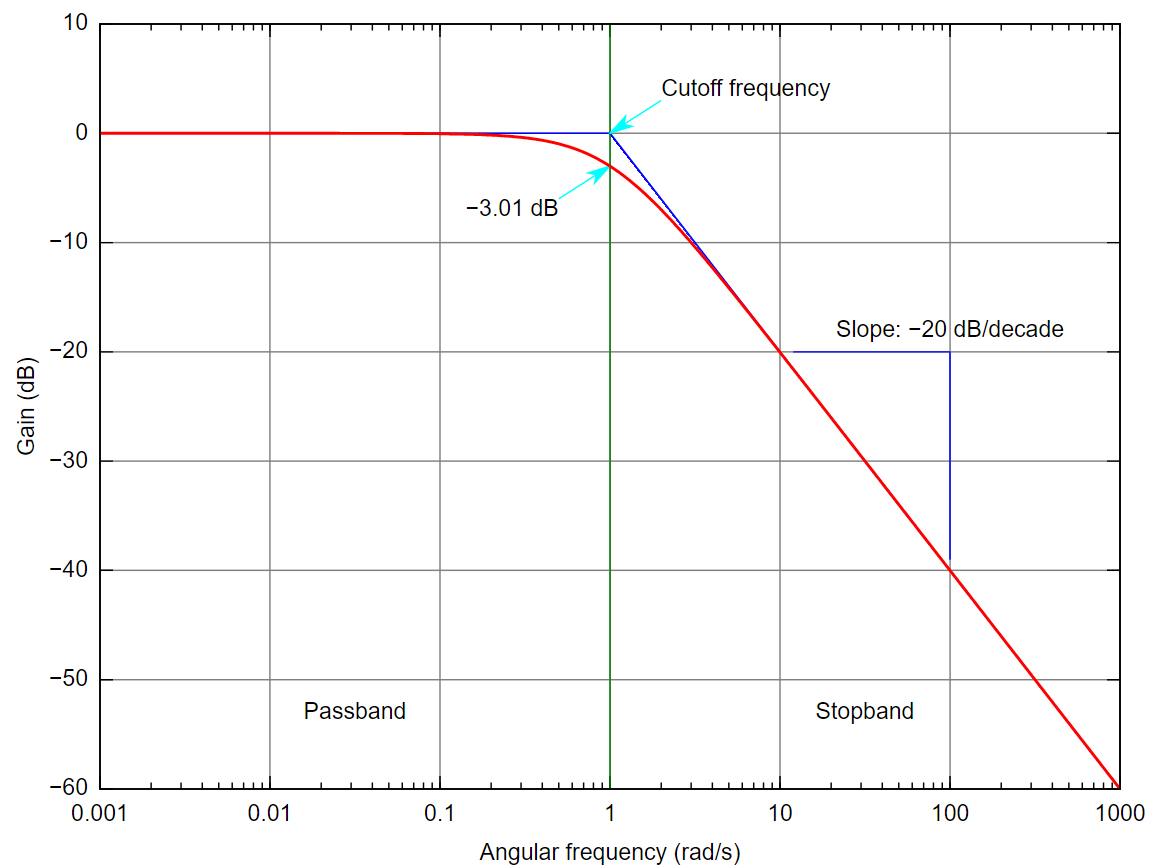
\includegraphics[scale = .5]{low_pass.png} %this is useful too \includegraphics[width = \linewidth]
	\caption{Example of Low Pass Filter: \url{https://upload.wikimedia.org/wikipedia/commons/6/60/Butterworth_response.svg}}
	\label{fig:lowpass}
\end{figure}    

In order to filter out higher frequencies in an audio signal transmission, we will build a low pass filter.  Specifically, we will describe how a low pass filter is created using a finite number of non-zero filter coefficients which is called a \textit{Finite Impulse Response} filter or FIR.  Given an impulse response, we can find the coefficients of the filter, and vice versa \cite{notes:class}.  For example, Figure \ref{fig:lowpass} shows a graphical depiction of a low pass filter that begins to cut out the frequencies above 1 rad/s.  Frequencies below the cutoff frequency are considered to be in the ``Passband," or allowable frequency band.  Frequencies above the cutoff frequency filtered out and are considered in the ``Stopband."  Ideally, the slope between the Passband and the Stopband would be as steep as possible to limit the passing of unwanted high audio frequencies.  The question still remains, how do you build a filter that eliminates these frequencies?  What is an impulse response?  Why do we need to find coefficients of a filter and what do they do?  Let's address those questions next. 

\subsubsection{Impulse Input, Impulse Response, and FFT}

	In our filtering example, we will be dealing with a Linear Time-Invariant (LTI) System.  A linear system is a class of systems where the system's outputs are the sum of the outputs of it's parts.  Additionally, Time-Invariant refers to a system where a time delay in the input sequence causes an equivalent delay in the output sequence.  Now, if we are given a LTI system, we can calculate everything about the system if we know the \textit{unit impulse response}.  The \textit{unit impulse response} refers to the system's time-domain output sequence when the input is a single unity-valued sample (unit impulse) surounded by zero-valued samples.  Furthermore, knowing the impulse response of an LTI system, the \textit{output sequence} is calculated by taking the \textit{convolution}  of the input sequence and the system's impulse response \cite{lyons:intro}.  We will talk more about convolutions later, but we typically do not perform convolutions in the time domain since they are computationally expensive.  Instead, multiplication is performed in the frequency domain.  In order to transform the impuse response into a \textit{frequency response}, we take the Fast Fourier Transform (FFT) of the impulse response\cite{lyons:intro}.

Let's explain with a simple example, if we let $x(n)$ be a discrete-time sequence of individual signal amplitudes, then we can define a simple LTI \textit{averager} system as follows: 

$$y(n) = \frac{1}{4} \left[ x(n)+x(n-1)+x(n-2)+x(n-3)\right] =  \frac{1}{4}\sum_{k=n-3}^{n} x(k)$$    

Given, this simple averager, we can show the block diagram in Figure \ref{fig:impulse} (a), impulse input and impulse response in Figure \ref{fig:impulse} (b), and the frequency magnitude response created from the FFT of the impulse response in Figure \ref{fig:impulse} (c).  The block diagram in Figure \ref{fig:impulse} (a) - also referred to as the \textit{Filter Structure}, simply shows how an impulse input is transformed into a impulse response.  The impulse response, $y(n)$, is created by passing the impulse input, $x(n)$, into the system and storing the four most recent values.  Once there are four values, they are added together and multiplied by $\frac{1}{4}$ to calculate the average.  The sequence proceeds one step averaging the most recent four values of the impulse input, $x(n)$, along the way.  Since there are four separate input sample values to calculate an output value, the structure of this filter can be referred to as a \textit{4-tap tapped-delay line FIR filter} using digital filter vernacular.  The coefficients of this filter are all $\frac{1}{4}$ and we can use an Fast Fourier Transform on the filter to provide all the frequency domain information.

\begin{figure}[h!]
	\centering
	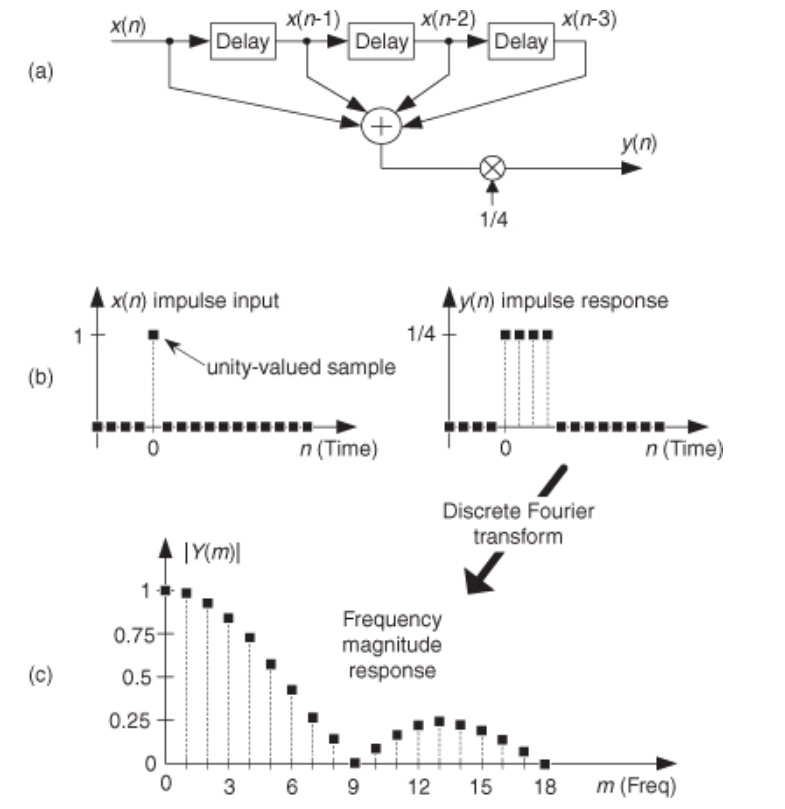
\includegraphics[scale = .6]{impulse.png} %this is useful too \includegraphics[width = \linewidth]
	\caption{Block Diagram (a), Impulse Input and Impulse Response (b), and Frequency Magnitude Response after FFT of Impulse Response (c).  Taken from Reference \cite{lyons:intro} below and is Figure 1-12 from Chapter 1}
	\label{fig:impulse}
\end{figure}    

From Figure \ref{fig:impulse} (c), the FFT transforms the impulse response $y(n)$ into $Y(m)$, which is the frequency domain information.  $Y(m)$ provides the frequency magnitude response of the simple 4-point averager.  This is actually an example of a low pass filter where the \textit{averager} reduces the amplitude (attenuates) the high-frequency  signal.  In our construction of a filter, we will have to use a different impulse response since we want to remove, not attenuate, the high frequency information content.  The following section will explain how we design a Finite Impulse Response (FIR) filter using the window method in order to create a low pass filter that removes high frequency information content. 

\subsubsection{Finite Impulse Response (FIR)}

An FIR filter has a finite duation of nonzero output values given a finite duration of input values (this is how they were named!).  Recall, in our example above, we used four ``taps" that were all equal to $\frac{1}{4}$.  The two factors that affect an FIR filter's frequency response are the number of taps and the coefficients\cite{lyons:intro}.  If we were to calculate the impulse response, $y(n)$, from the impulse input, $x(n)$, in the time-domain, then we would have to perform the mathematical operation of a convolution.  More specifically for an \textit{M}-tap filter, we would calculate $y(n)$ as follows: 

$$y(n) = \sum_{k=0}^{M-1}  h(k)x(n-k)$$

Where $h(k)$ are the filter coefficients for each of the taps.  \textbf{The terms FIR filter coefficients and impulse response mean the same thing}\cite{lyons:intro}.  We can re-write the above equation using \textit{convolution} notation as follows: 

$$y(n) = h(k) \star x(n)$$  

The major concept is that convolution in the time domain is equal to multiplication in the frequency.  The process in which we can move from one domain to the other is through the Fast Fourier Transform (FFT).  The FFT of $y(n)$ is equal to $Y(m) = H(m) X(m)$, which is the spectrum of the filter output.  In a similar way, we can determine $h(k)\star x(n)$ by taking the inverse of the FFT (we will denote this as IDFT - Inverse Discrete Fourier Transform)\cite{lyons:intro}.  The important relationships are as follows: 

\begin{enumerate}
\item $x(n) \overset{FFT}{\longrightarrow} X(m)$
\item $X(m) \overset{IDFT}{\longrightarrow} x(n)$
\item $h(k) \overset{FFT}{\longrightarrow} H(m)$
\item $H(m) \overset{IDFT}{\longrightarrow} h(k)$
\item $y(n) \overset{FFT}{\longrightarrow} Y(m) \Rightarrow h(k)\star x(n) \overset{FFT}{\longrightarrow} H(m) X(m)$
\item $Y(m) \overset{IDFT}{\longrightarrow} y(n) \Rightarrow H(m) X(m) \overset{IDFT}{\longrightarrow} h(k)\star x(n)$
\end{enumerate}    

Now that we can easily move between the frequency and time-domains using the FFT or IDFT, let's design our own low-pass filter by determining the desired frequency response and moving back to the time domain through an IDFT to calculate the filter coefficients that will provide the desired frequency response.  Recall, in our hearing test example, our project group was unable to hear any frequency information content above 15kHz.  As such, we will attempt to design a low-pass filter that removes all of the frequency content above this threshold.  Therefore, our \textit{cutoff} frequency is 15kHz (see Figure \ref{fig:lowpass} for a depiction of the cutoff frequency).  To design the filter, we define the  \textbf{Frequency Cut-off Values} (End of Pass Band and Beginning of Stop Band), the \textbf{Sample Rate}, and the \textbf{Stop Band Attenuation} (in Decibels), and then use a Filter Design Tool within the GNU Radio application (which is written in Python) to apply the inverse FFT function to get the FIR filter coefficients.  

\begin{figure}[h!]
	\centering
	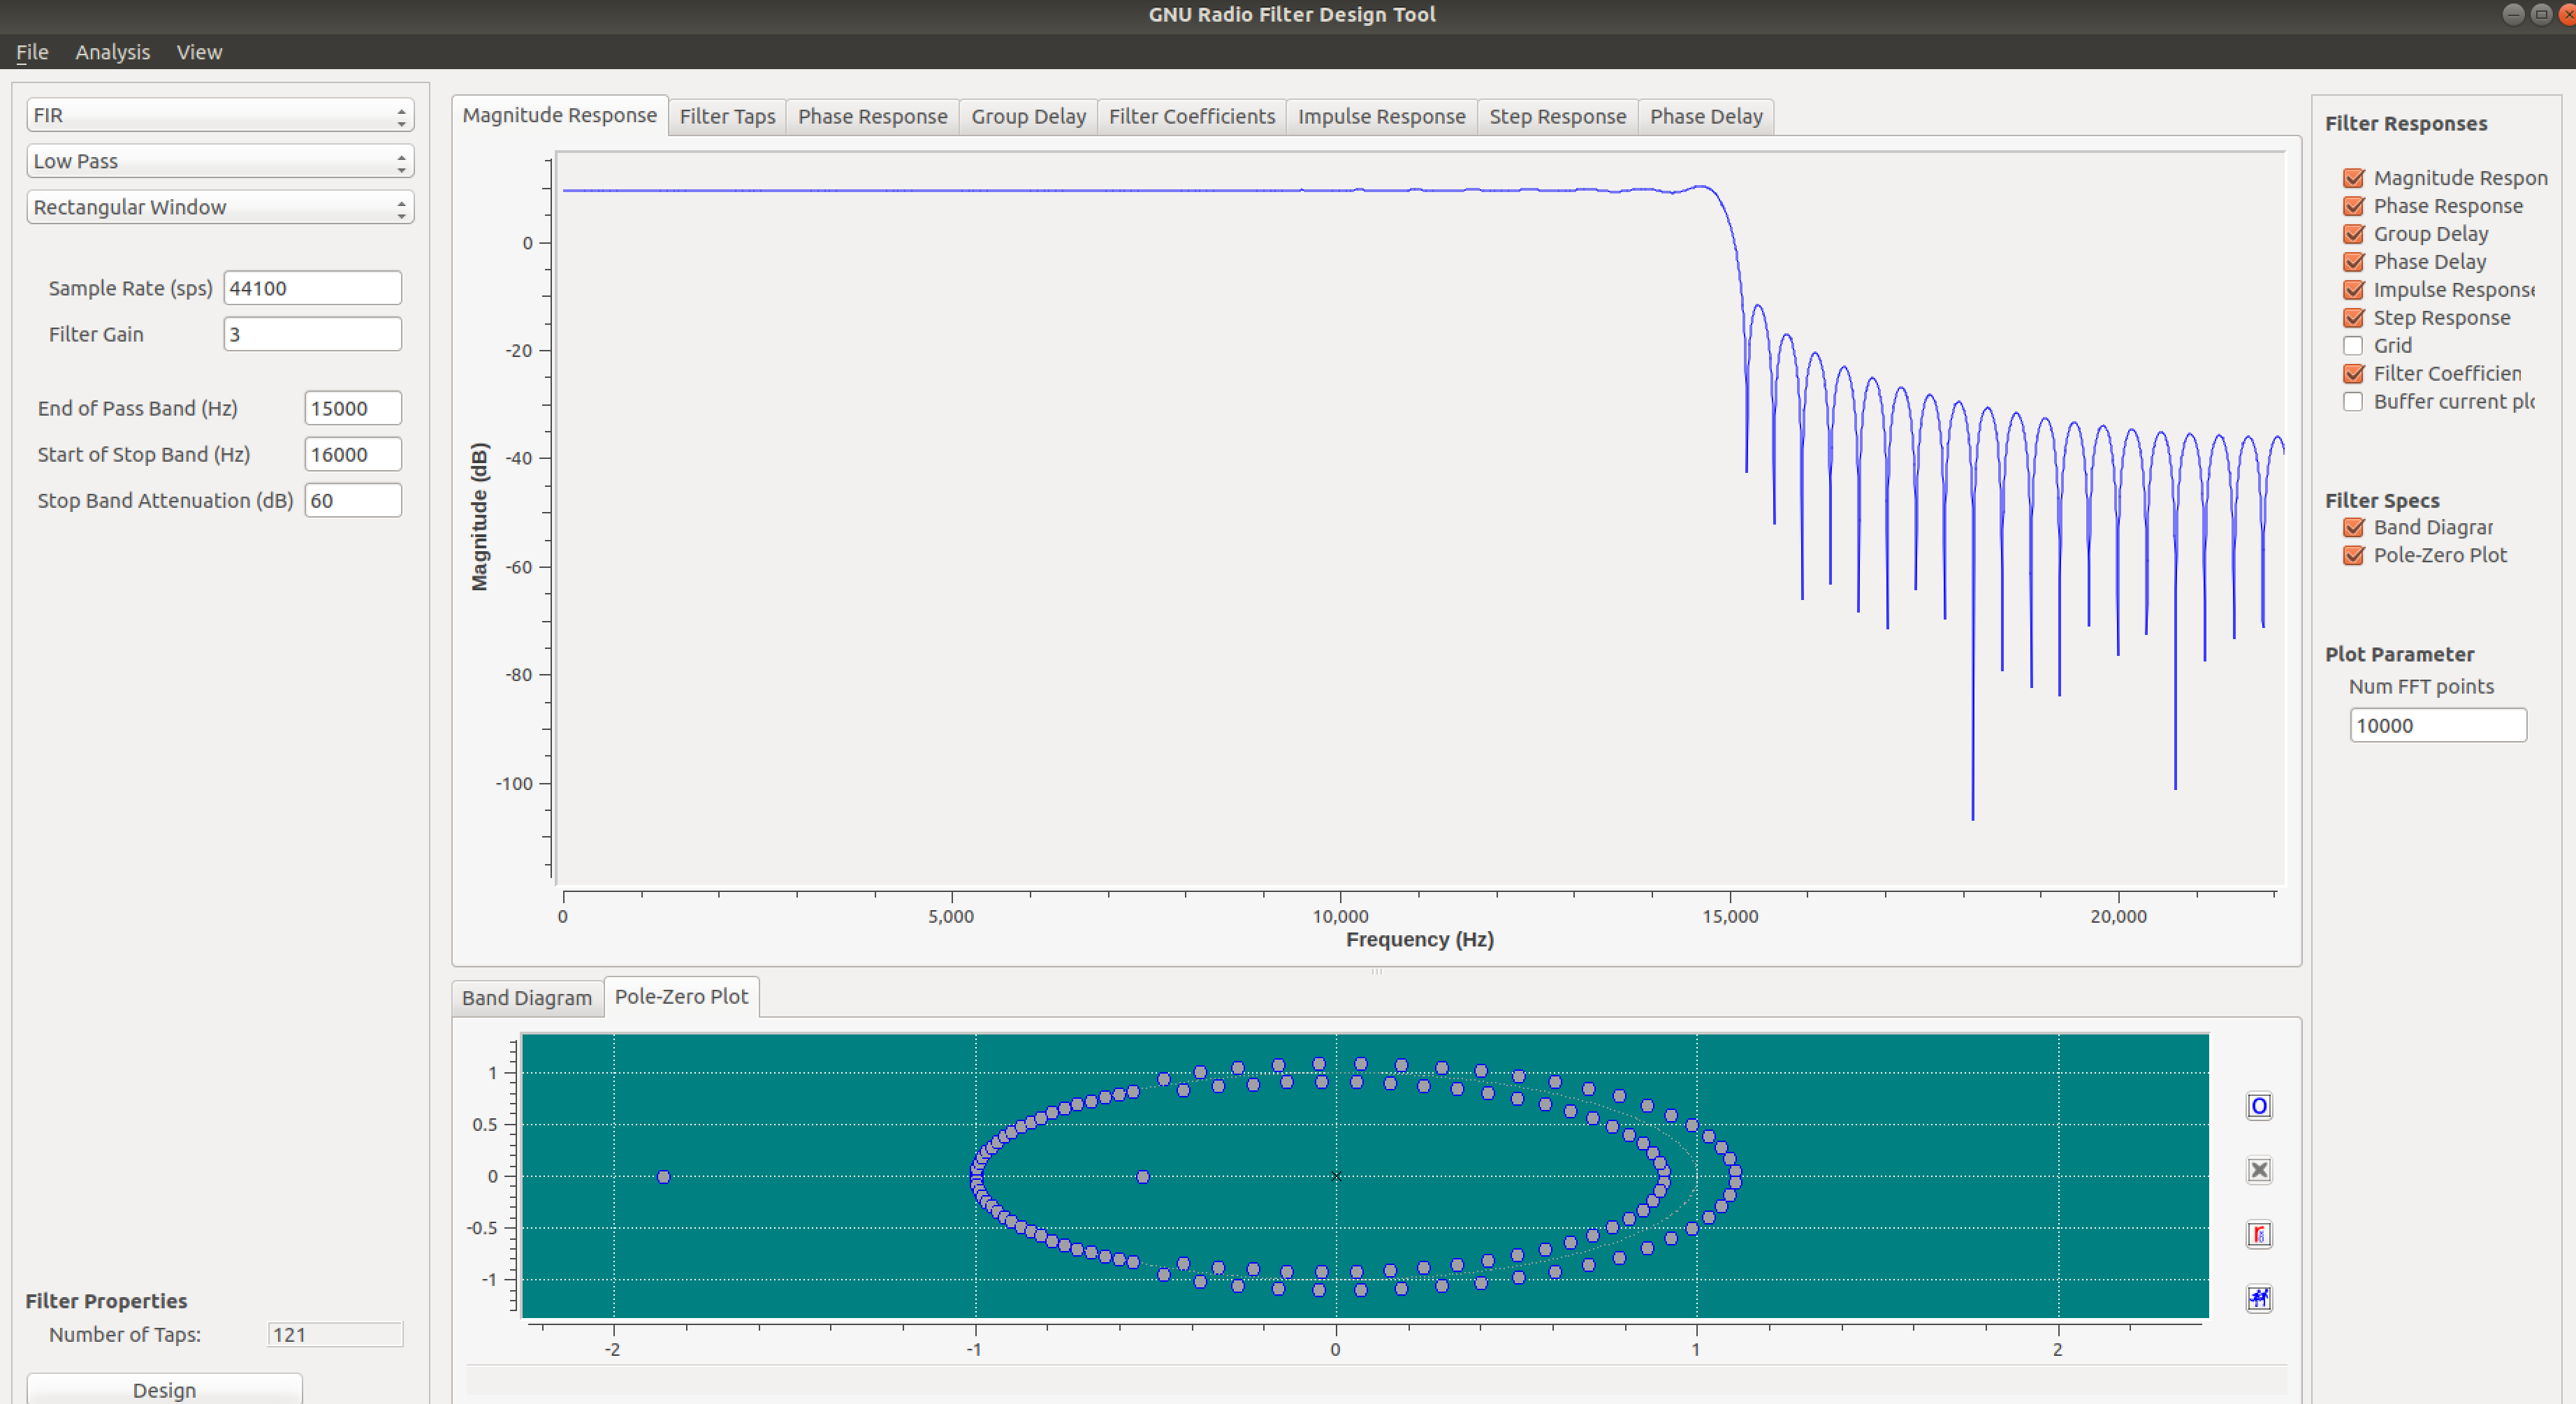
\includegraphics[height = 5cm, width =9cm]{filter_tool_15kHz.png} %this is useful too \includegraphics[width = \linewidth]
	\caption{Designing the 15kHz Filter using the Filter Design Tool within GNU Radio}
	\label{fig:mainfilt}
\end{figure}  

We set the Sample Rate $= 44,100$, the End of the Pass Band at  $15,000$ kHz, the Beginning of the Stop Band at $16,000$, and the Stop Band attenuation at $60$ dB.  After hitting the ``Design" button, the Frequency Response is displayed in Figure \ref{fig:mainfilt}.  As expected, the frequency response shows a drop-off at 15kHz where the Pass Band ends and the frequencies are cut.  The tool will use the frequency response created in order to generate the filter coefficients, or taps.  Figure \ref{fig:taps15} shows the filter coefficients that take the shape of a Sinc function.  The filter coefficients are saved and then passed into the GNU Radio Tool that implements the filter created.      

\begin{figure}[h!]
	\centering
	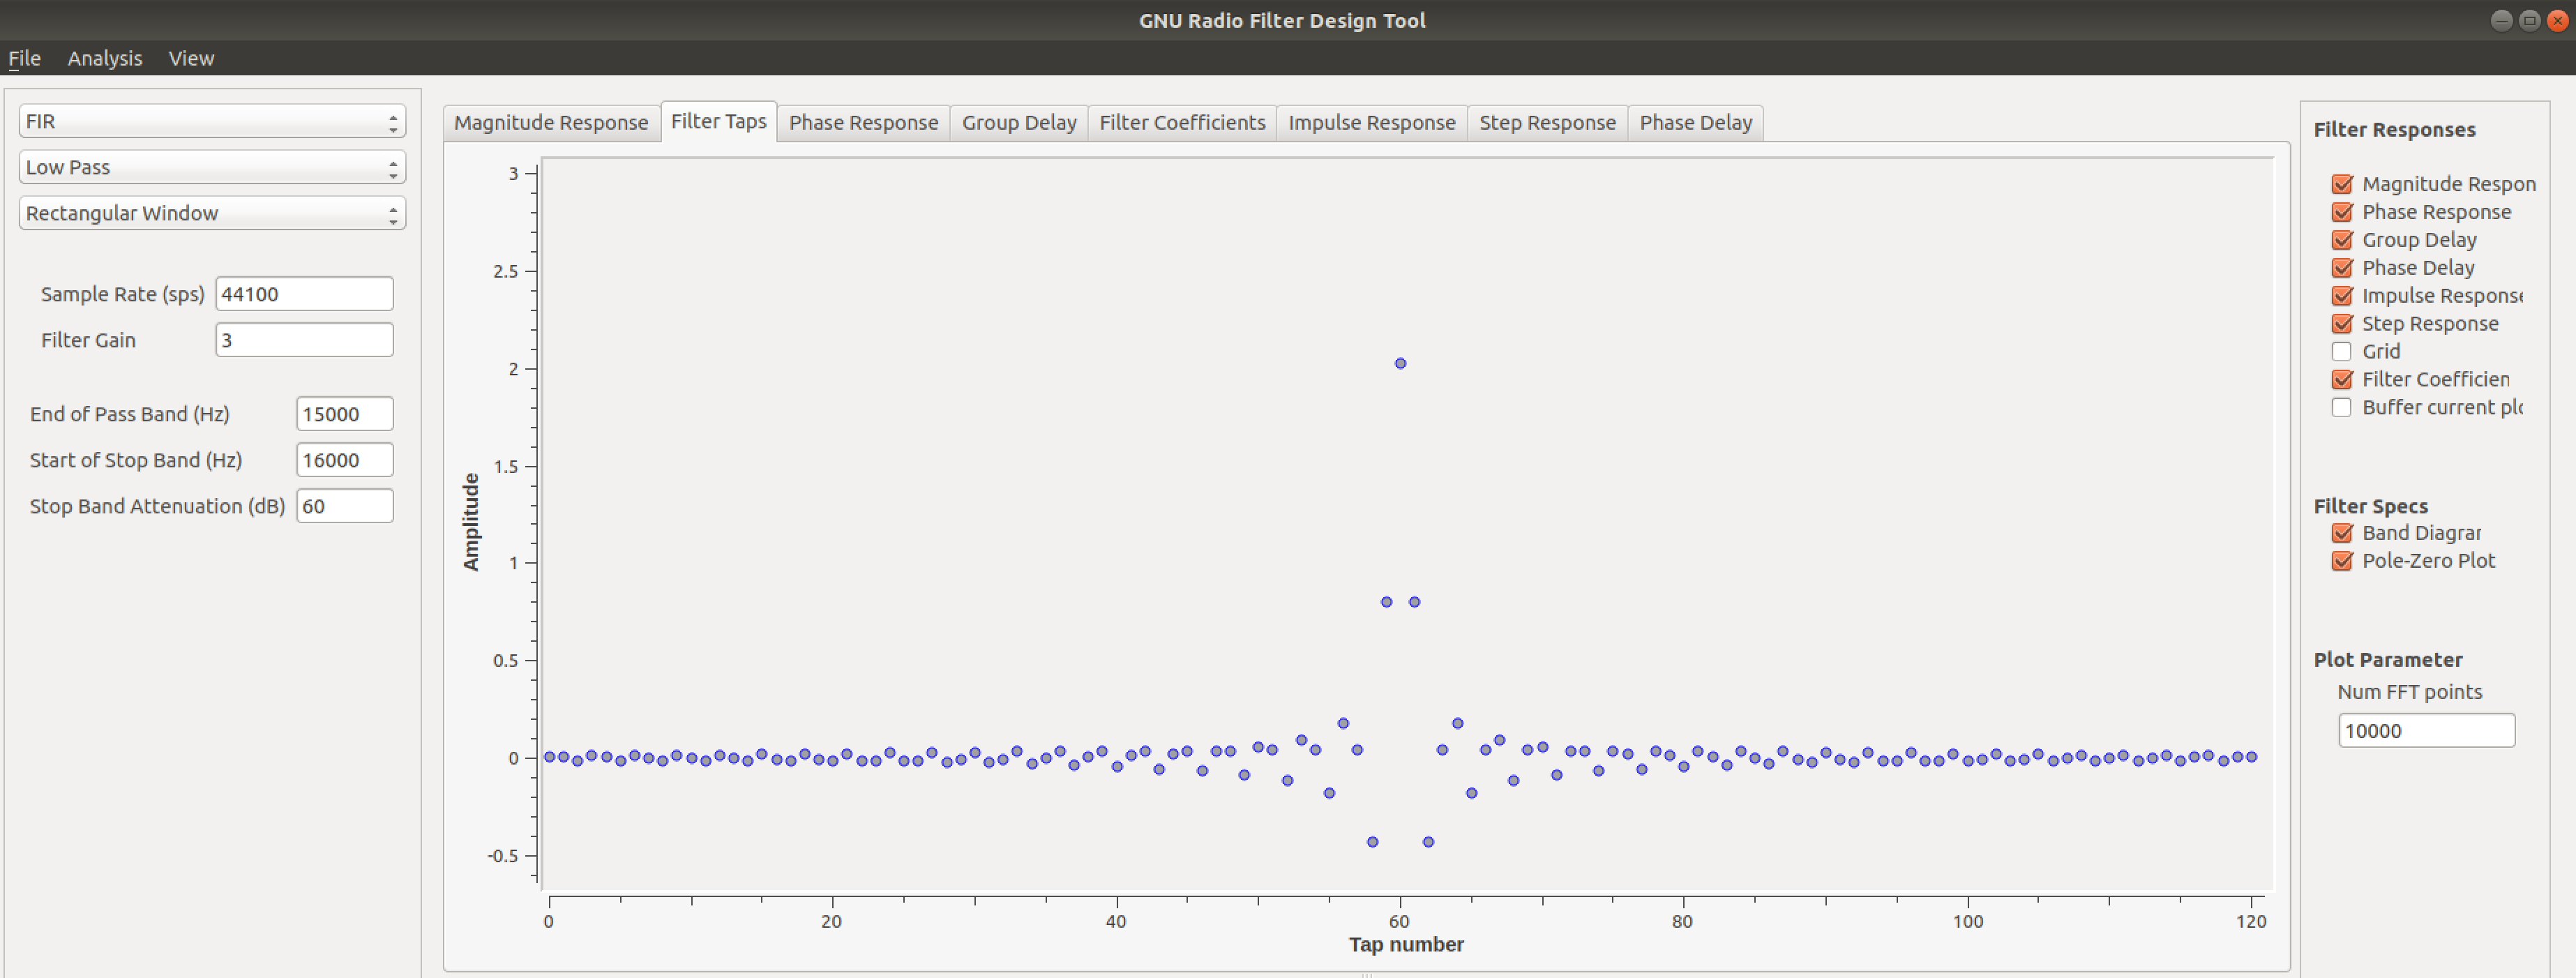
\includegraphics[height = 5cm, width =9cm]{filter_tool_15kHz_taps.png} %this is useful too \includegraphics[width = \linewidth]
	\caption{Filter Coefficients for the 15kHz Filter using the Filter Design Tool within GNU Radio}
	\label{fig:taps15}
\end{figure}   
  
 

\subsection{Nyquist-Shannon Sampling Theorem}

When recording audio signals, one has to set a sampling rate
(rate for analog signal, frequency for discrete signal). There
are several reasons why we set a sampling rate:

\begin{enumerate}
	\item Data storage conservation,
	\item Bandwidth conservation,
	\item Power conservation.
\end{enumerate}

The formula for sampling is:

\begin{equation}
	x[n]=x(t)|_{t=nT_{S}}=x(nT_{S})
	\label{eqn:signal}
\end{equation}

Where \(T_{S}\) is the sampling period and \(f_{S}=
\dfrac{1}{T_{S}}\) is the sampling frequency 
\cite{notes:class}. Lastly, $n$ is an index of the samples.

However, we have to be careful not to set this sampling rate too
low, or else we run into a problem called aliasing. Low-frequency
aliasing is caused by undersampling, and occurs when a different
time function with a lower frequency produces the same set of
samples \cite{aliase:wiki}. For example, the signal produced by
the function:

\begin{equation}
	x[t]=cos(2\pi10t)
\end{equation}

can be visualized (in the time domain) as:

\begin{figure}[H]
	\centering
	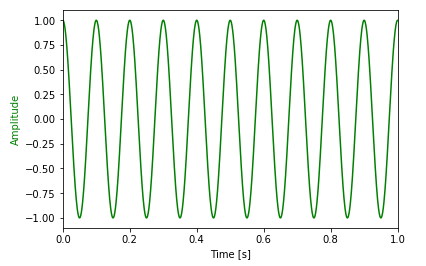
\includegraphics[scale = 1]{images/original_signal.png} %this is useful too \includegraphics[width = \linewidth]
	\caption{Original signal, from equation \ref{eqn:signal} \cite{notebook:sampling}.}
	\label{fig:signal_og}
\end{figure}    

Converting to a discrete signal, by undersampling at 18 Hz rate, we
produce the aliasing, as can be seen below.

\begin{equation}
	x[n]=\cos(\frac{2\pi \cdot 10n}{18})
\end{equation}

Because the signal is periodic, adding or subtracting $2\pi n$ 
inside of the cos function does not change the equation.

\begin{equation}
	x[n]=\cos(\frac{10\pi \cdot n}{9} - 2\pi n)
\end{equation}
\begin{equation}
	x[n]=\cos(\frac{10\pi \cdot n}{9} - \frac{18\pi n}{9})
\end{equation}
\begin{equation}
	x[n]=\cos(-\frac{8\pi\cdot n}{9})
\end{equation}
\begin{equation}
	x[n]=\cos(\frac{8\pi\cdot n}{9})
\end{equation}

By undersampling, we create an alias signal corresponding to
\(8\pi\dfrac{n}{9}\). Our sample rate of 18 Hz is too low. Below
is our sampling overlaid on the original curve.

\begin{figure}[H]
	\centering
	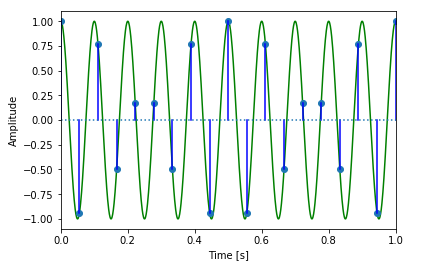
\includegraphics[scale = 1]{images/sub_sample.png} %this is useful too \includegraphics[width = \linewidth]
	\caption{
		Overlaid sampling (in blue) on the original curve (in green) 
		\ref{eqn:signal} 
		\cite{notebook:sampling}.
	}
	\label{fig:sub_sample}
\end{figure}    

This shows that that there are additional functions that can cross
through the sampling points of our original signal, creating
alternative interpretations. For example, in the graph below,
notice that the red curve matching the aliased result is a valid
interpretation of the sampled points originally derived from the
green curve.

\begin{figure}[H]
	\centering
	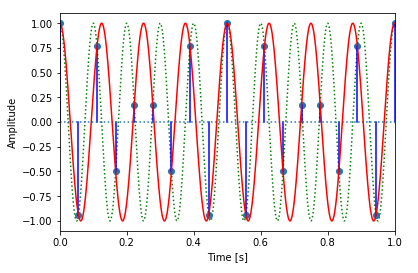
\includegraphics[scale = 1]{images/aliased_curve.png} %this is useful too \includegraphics[width = \linewidth]
	
 \caption{
	The aliased signal (in red) intersects the original
 	signal (in green) at the sampling points (in blue)
	\ref{eqn:signal} \cite{notebook:sampling}.
	} 
 	\label{fig:aliase}  
 \end{figure}

So, if our objective is to sample as little as possible, how do
we determine the minimum rate necessary? The Nyquist-Shannon theorem states that if a function $x ( t )$ contains no
frequencies higher than $B$ hertz, then it is completely determined by
giving its ordinates at a series of points spaced $1 / ( 2 B )$
seconds apart \cite{shannon:wiki}. It then follows that a sufficient sampling rate (nyquist rate) is therefore twice the maximum frequency $B$ Hz, $2B$ \cite{shannon:wiki}.
Restated from a different angle: for a given sample rate $f_{s}$, perfect reconstruction of a signal is guaranteed for a bandlimit $B<f_{s}/2$ \cite{shannon:wiki}.


In our case, before processing with a filter, our raw signal had
a sampling rate of 44.1 kHz. This is the standard for CD-quality
audio. Since human hearing range is roughly 20 Hz to 20,000 Hz, the sampling rate has to at least be 40 kHz (from the Nyquist-Shannon theorem). Audio signals still have to be passed through a low-pass anti-aliasing filter, because even though humans cannot hear frequencies beyond that, these signals can still cause aliasing. A transition band of 4,100 Hz is added to the 40 kHz allows greater ease of anti-aliasing filtering \cite{cd:wiki}. Figure \ref{fig:lowpass} shows this transition band.  The larger this band, the less 'sharp' of a filter is required. This results in the standard frequency of 44.1 kHz for CDs.



We know from Equation \ref{eqn:nyq} that the maximum
frequency that can be represented at any given sampling rate is
half the sampling rate; thus a 44.1 kHz CD can capture tones up
to 22.05 kHz. This is often over-kill, since as previously
mentioned, humans often cannot hear beyond 15 kHz. We have space
to trim that down, but we must make sure to use filters to
prevent aliasing.

\section{Evaluation of Filtered Signal}

To demonstrate the effects of low-pass filtering on a
digitally-sampled audio file, we have built an application using
the GNU Radio development framework. In addition to filtering and
playing audio, the application demonstrates the importance of
bandwidth reduction by transmission of the processed audio using
a pair of software-defined radios operating at 903 MHz.

The GNU Radio project \cite{GNU:radio} is an open-source toolkit
supporting the development of software-defined radios. Typically,
application developed by building a flowgraph consisting
of signal-processing components or "blocks" and their interconnects.  

Once the flowgraph is designed, the layout is automatically
converted into a Python program that manages the GNU Radio
scheduler. The scheduler efficiently manages the routing of the
work products to-and-from each block and is not limited by the
speed of the Python interpreter. The signal-processing components
are usually coded in C++ (for performance reasons).

\subsection{Demo Flowgraph Overview}
Our flowgraph is shown in figure \ref{fig:flowgraph} and the
automatically-generated Python code is provided in the Appendix
(Listing \ref{lst:demo}). Note that the interconnected blocks
have multi-colored input and output tabs. The blue tabs show that
the block produces or consumes a complex number, while the orange
tabs indicate the use of simple floating-point values. Input tabs
may only connect to one output tab, but output tabs may connect
to one-or-more input tabs. Every tab must be connected.  

Certain components have no connections.  Primarily these blocks
represent parameter blocks and are used to simplify the layout of
the flowgraph.  The blocks with the labels starting with "QT" 
represent graphical-user interface (GUI) elements that will be 
shown when the application is run.  Our application uses the 
following GUI elements:

\begin{itemize}
	\item Source selection (radio buttons)
	\item Filter selection (radio buttons)
	\item Volume (slider)
	\item Amplitude vs Time (oscilloscope widget)
	\item Amplitude vs Frequency (spectrograph widget)
\end{itemize}

\subsection{Sources}

Three sources are defined for the demo. The first source is
"silence", which is generated by a constant stream of zeros. 

The second source is simply a two-tone signal using 440 Hz (A
above middle C), which is the reference frequency for the
standard musical scale, and 3520 Hz, which is three octaves above
the first tone. When selected in the demo, these two tones
provide a very clear indication of the effects of the 1-kHz
filter.

The third source is a digitally-sampled, CD-quality
snippet from a recording of a performance of "Flight of the
Bumblebee". With an effective bandwidth of 22.05 kHz, this source
is affected by all of the filters. The block is set to
"loop", so that it will run continuously.

A \textit{QT GUI Chooser} drives the source selection block,
allowing the chosen signal to pass to the rest of the flowgraph
while blocking the other two sources.

\subsection{Filter}
Five filter options are defined: 
\begin{itemize}
	\item No filter
	\item 15-kHz filter
	\item 8-kHz filter
	\item 4-kHz filter
	\item 1-kHz filter
\end{itemize}

The filters are implemented using the \textit{FFT Filter} component, which
implements a lowpass filter by taking the Fourier Transform of the
incoming signal, multiplying that by the transfer function
representing the filter, and then performing an inverse-FFT to
generate the output waveform.  The filter parameters are given to 
the block as a sequence of filter taps, as defined above.

As in the source selection, the filter selection is managed by a
QT GUI chooser block driving a selector block.  The output of the 
selector block continues to the rest of the flowgraph.

\subsection{Instrumentation}
In order to visualize the operation of the filters, two GUI elements
are used: an oscilloscope-like widget that charts amplitude versus time,
and a spectrograph-like widget that shows amplitude versus frequency.
When the different filters are chosen, the spectrograph clearly shows
the change in bandwidth of the signal.

\subsection{Output}

Local audio output is provided by an \textit{Audio Sink} block
that drives the default audio device of the computer on which the
program is run. The volume slider controls a multiplier block
that directly affects the amplitude seen by both the and \textit{Audio
Sink} and the radio.

An amplitude-modulation (AM) radio is created in order to
demonstrate a primary benefit of lowpass filtering: radio
transmission bandwidth reduction. The operation of the AM-radio
portion of the flowgraph is beyond the scope of this paper, but
the output drives a software-defined-radio peripheral that
transmits the audio at a center frequency of 903.5 MHz, which is
500 kHz above the base frequency of the radio.

\subsection{Results}

The GNU Radio toolkit provided a very effective platform for
demonstrating the effects of lowpass filtering of different audio
sources. Though not rigorously tested, we observed the behavior
that was expected: the 15-kHz and 8-kHz filters reduced the
bandwidth of the signal, but it was not readily discernible to
our ears. It wasn't until we selected the 4-kHz filter that a
difference was clearly noted.

\begin{figure*}
	\centering
	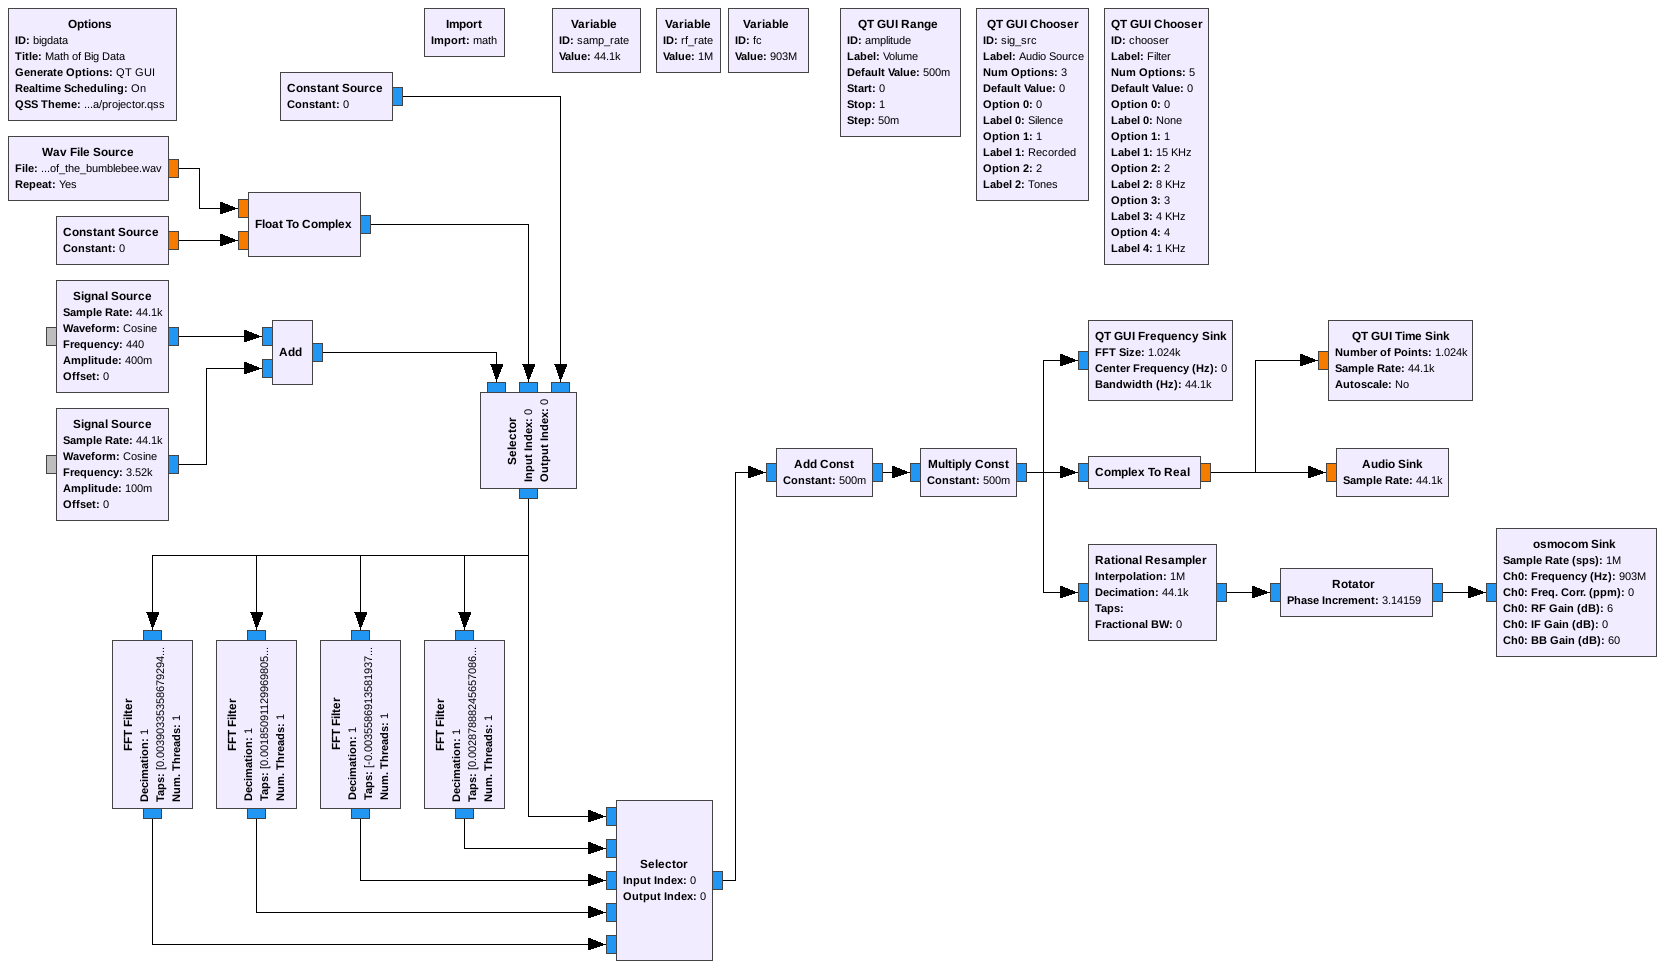
\includegraphics[width=\textwidth]{images/player_grc.png} 
	\caption{Demonstration Application Flowgraph}
	\label{fig:flowgraph}
\end{figure*}    

\begin{figure}
	\centering
	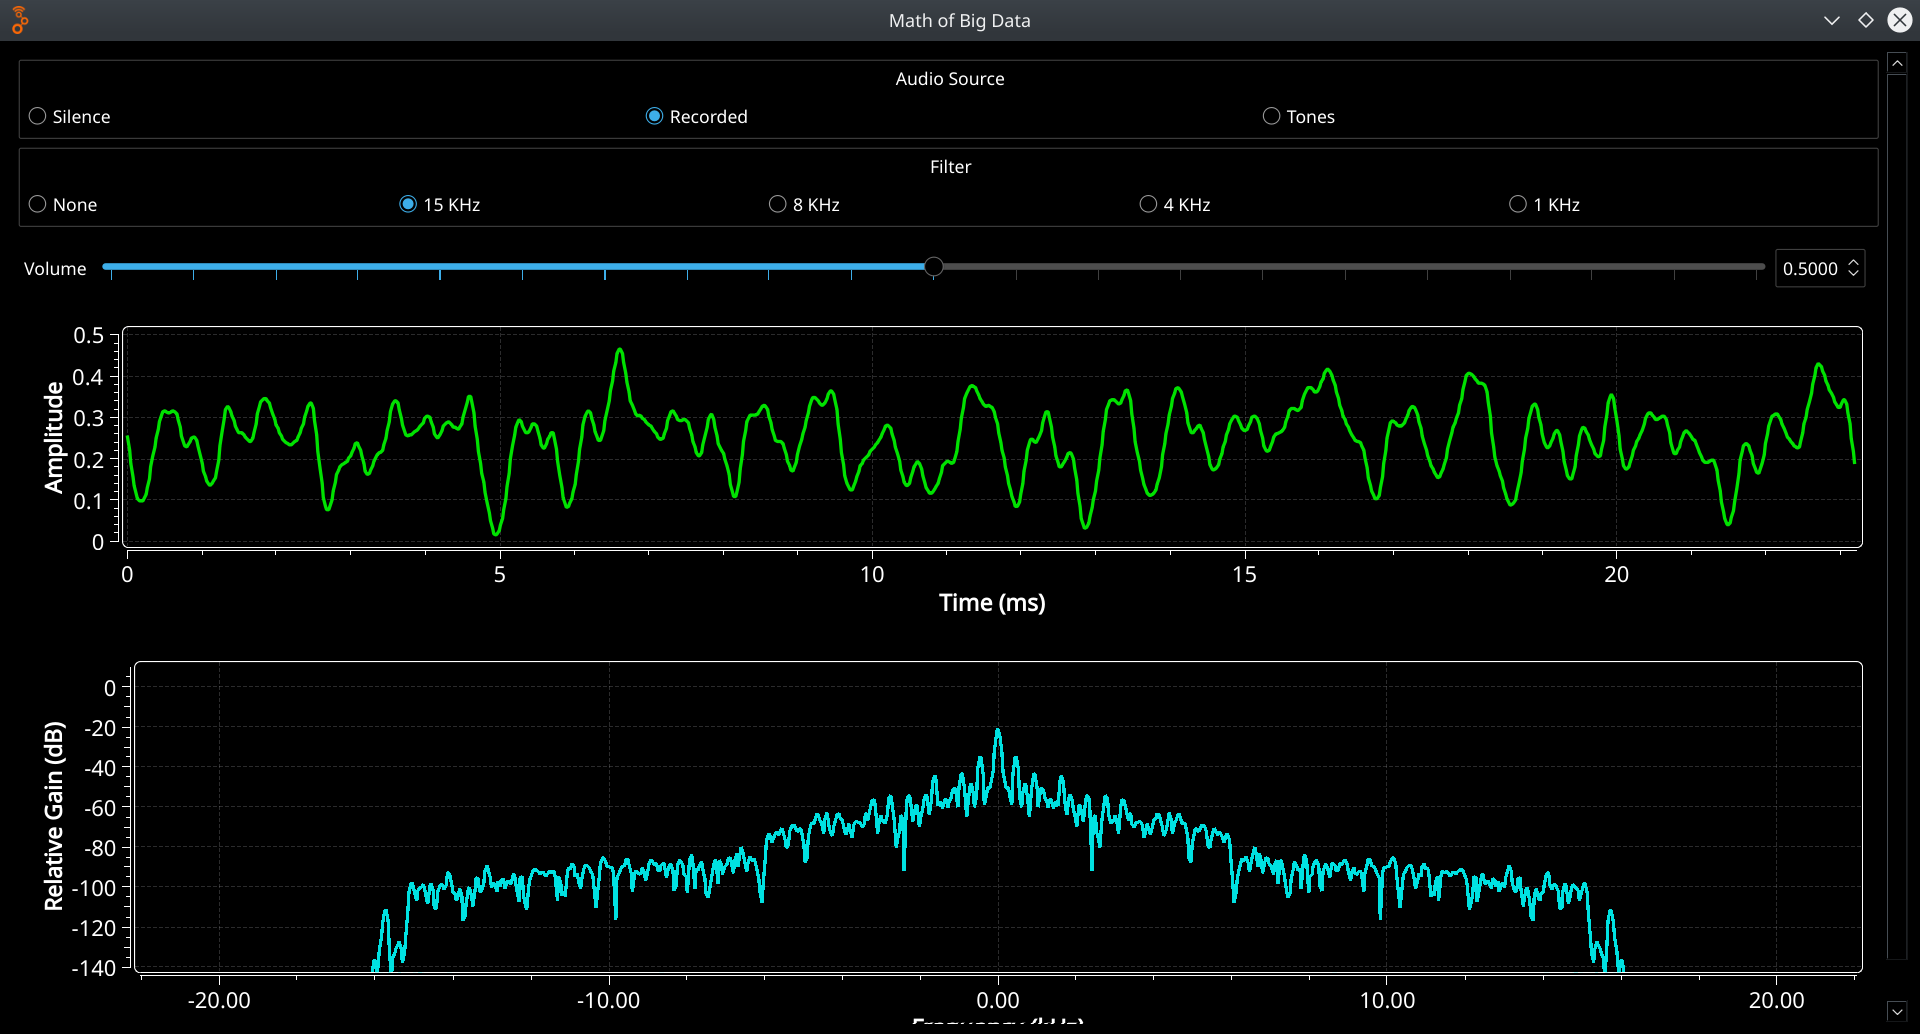
\includegraphics[width=\linewidth]{images/application.png} 
	\caption{Demonstration Application: 15 kHz Filter}
	\label{fig:fifteen}
\end{figure}    

\begin{figure}
	\centering
	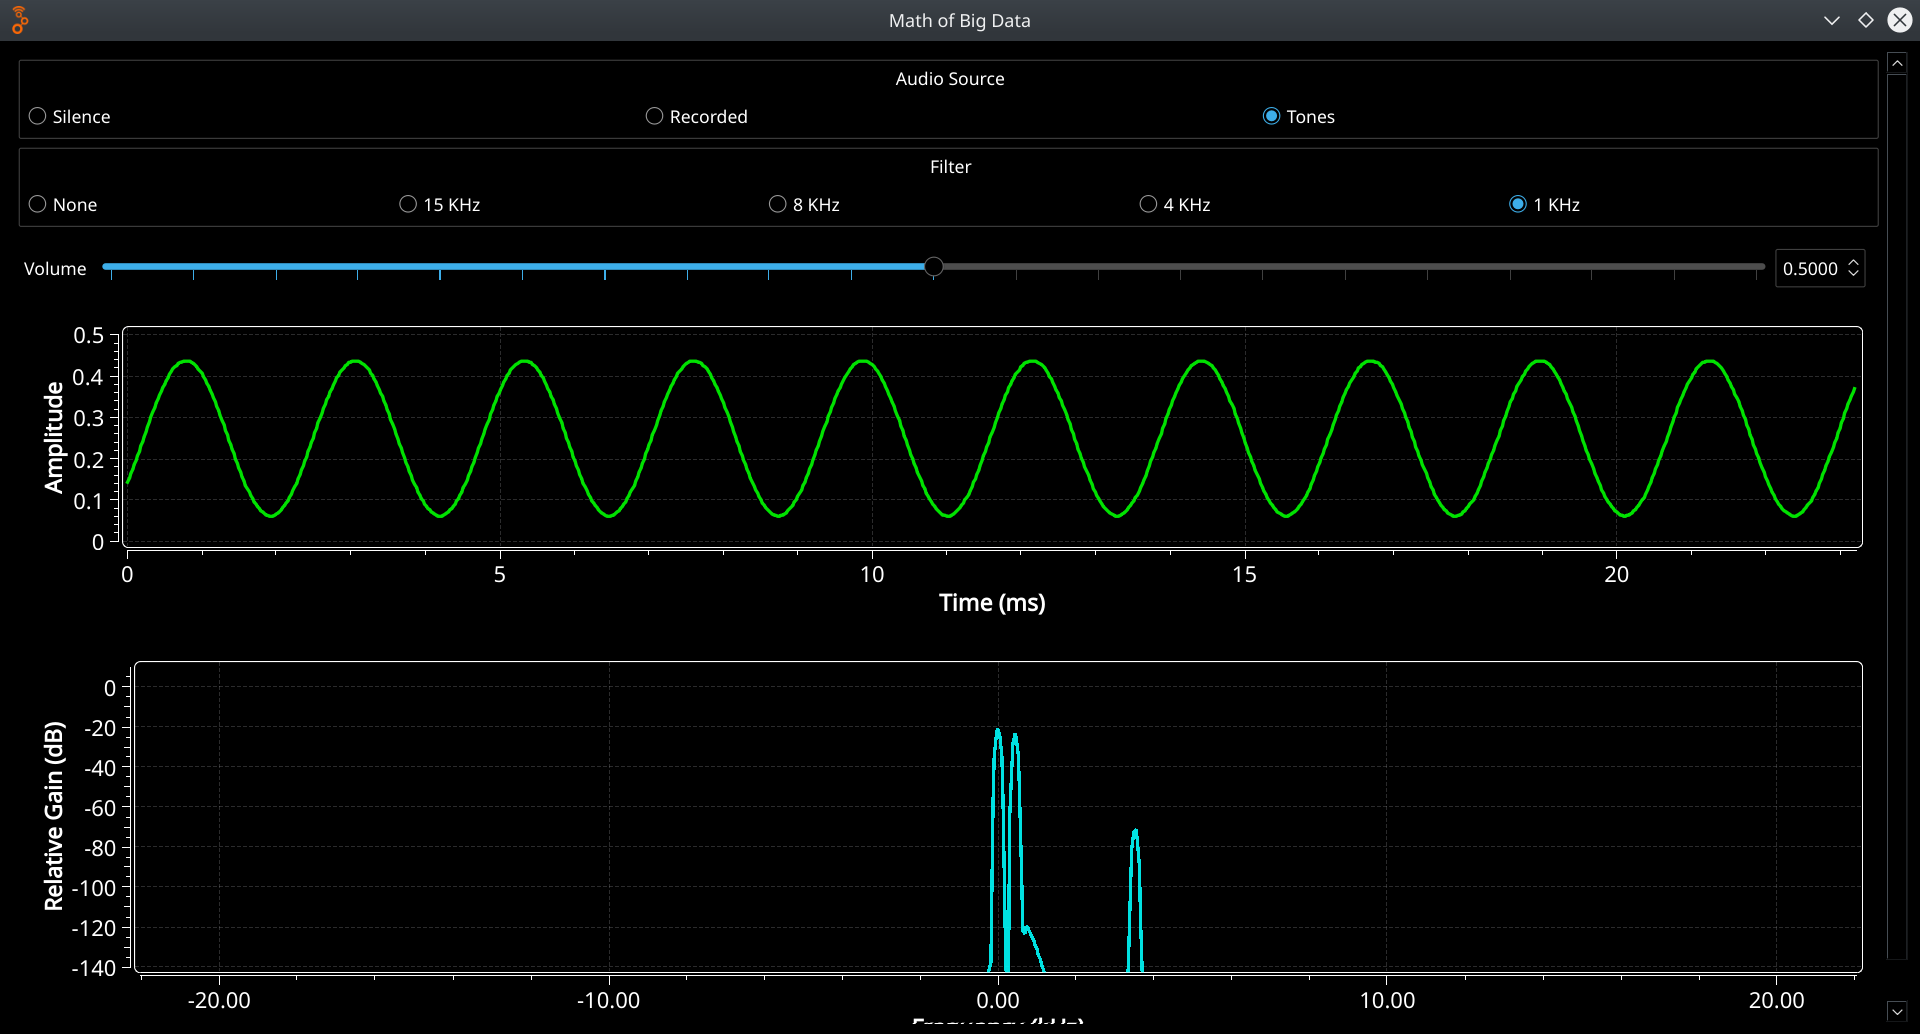
\includegraphics[width=\linewidth]{images/application2.png}
	\caption{Demonstration Application: 1 kHz Filter, Tones}
	\label{fig:tones}
\end{figure}    

\section{Conclusion}
The conclusion goes here.


\begin{thebibliography}{1}

\bibitem{GNU:radio}
\emph{GNU Radio}, \url{https://www.gnuradio.org/}.

\bibitem{notes:class}
Baxley, R., Henshaw, A., Nowlan, S., \& Trewhitt, E. \emph{Software-Defined Radio with GNU Radio: Theory and Application, Georgia Tech Professional Education course notes.} (2017)

\bibitem{human:rg}
Rossing, Thomas (2007). Springer Handbook of Acoustics. Springer. pp. 747, 748. ISBN 978-0387304465.

\bibitem{lyons:intro}
Lyons, Richard G. Author. "Understanding Digital Signal Processing."  Ch. 1, 3, and 5. Web.

\bibitem{lowpass:wiki}
\url{https://en.wikipedia.org/wiki/Low-pass_filter}.  Accessed Nov. 7, 2019.

\bibitem{harris:rot}
Harris, Fred J. "Multirate Signal Processing for Communication Systems." Page 216, Equation 8.16.

\bibitem{aliase:wiki}
\url{https://en.wikipedia.org/wiki/Nyquist_frequency}.  Accessed Nov. 15, 2019.

\bibitem{notebook:sampling}
Baxley, R., Henshaw, A., Nowlan, S., \& Trewhitt, E. \emph{Juyter Notebook for Sampling: Sampling.ipynb.} (2017)

\bibitem{sinc:wiki}
\url{https://en.wikipedia.org/wiki/Nyquist_frequency}.  Accessed Nov. 16, 2019.

\bibitem{shannon:wiki}
\url{https://en.wikipedia.org/wiki/Nyquist\%E2\%80\%93Shannon_sampling_theorem}.  Accessed Nov. 20, 2019.

\bibitem{cd:wiki}
\url{https://en.wikipedia.org/wiki/44,100_Hz}. Accessed Nov. 20, 2019.

\end{thebibliography}


\newpage


\onecolumn
\appendix 

\subsection{Python Code for Filter Design\cite{notes:class}}

\lstinputlisting[language = Python]{filter.py}

% that's all folks
\end{document}


